% id: 101-01
% book: 개념원리 중학 3-2 · 11 접선과 현이 이루는 각
% section: 개념원리 확인하기
% figure: crop:fig-101-01.png
% answer: ⑴ ○ ⑵ × ⑶ × ⑷ ○
% answer_source: 답지
% variant_level: 0 (원본 전사)
% 이 파일은 build.mjs 가 items.json 에서 만든다. 고칠 때는 items.json 을 고친다.
\smash{\raisebox{1.5mm}{\dmkichul{개념원리 중학 3-2 101쪽 01번}}}
\noindent\begin{minipage}[t]{0.58\linewidth}\vspace{0pt}\raggedright 오른쪽 그림에서 직선~$\pt{TT'}$은 원의 접선이고 점~$\pt{B}$는 접점일 때, 다음 중 옳은 것은 ○, 옳지 않은 것은 ×를 (\quad) 안에 써넣으시오.\end{minipage}\hfill\begin{minipage}[t]{0.4\linewidth}\vspace{0pt}\centering \setlength{\dmfigw}{78.5pt}\ifdim\dmfigw>\linewidth\setlength{\dmfigw}{\linewidth}\fi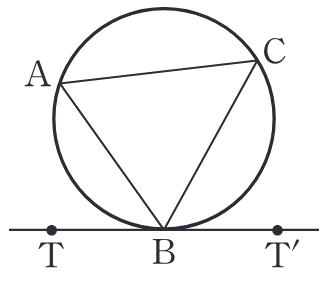
\includegraphics[width=\dmfigw]{figures/fig-101-01.png}\end{minipage}\par
\dmsubprob{1} $\angle\pt{ABT}=\angle\pt{ACB}$\nobreak\hfill\mbox{(\qquad)}
\dmsubprob{2} $\angle\pt{ACB}=\angle\pt{CBT'}$\nobreak\hfill\mbox{(\qquad)}
\dmsubprob{3} $\angle\pt{CAB}=\angle\pt{ABT}$\nobreak\hfill\mbox{(\qquad)}
\dmsubprob{4} $\angle\pt{CBT'}=\angle\pt{CAB}$\nobreak\hfill\mbox{(\qquad)}
